對於有許多條件語句(通常是\texttt{if()}語句)的程序,分支預測的有效性通常決定了整體性能。如果準確地預測分支,那麼在分支上基本上沒有任何開銷。要是分支預測有一半是錯誤的,可能會比常規算術指令慢十倍或更多。

硬件分支預測是基於處理器執行的條件指令。因此,處理器對條件的理解可能與我們不同。下面的例子有助於我們理解這一點:

\hspace*{\fill} \\ %插入空行
\noindent
\textbf{02\_branch.C}
\begin{lstlisting}[style=styleCXX]
std::vector<unsigned long> v1(N), v2(N);
std::vector<int> c1(N), c2(N);
for (size_t i = 0; i < N; ++i) {
	v1[i] = rand();
	v2[i] = rand();
	c1[i] = rand() & 0x1;
	c2[i] = !c1[i];
}
unsigned long* p1 = v1.data();
unsigned long* p2 = v2.data();
int* b1 = c1.data();
int* b2 = c2.data();
for (auto _ : state) {
	unsigned long a1 = 0, a2 = 0;
	for (size_t i = 0; i < N; ++i) {
		if (b1[i] || b2[i]) { // !!!
			a1 += p1[i];
		} else {
			a1 *= p2[i];
		}
	}
	benchmark::DoNotOptimize(a1);
	benchmark::DoNotOptimize(a2);
	benchmark::ClobberMemory();
}
\end{lstlisting}

有趣的是\texttt{if (b1[i] || b2[i])}條件:計算總為\texttt{true},因此可以期待處理器的完美預測。當然,事情沒這麼簡單。從邏輯上,看起來這一個單獨的條件,但對從CPU角度來說,是兩個獨立的條件分支:一半的情況下,在第一個分支,總體結果正確;另一半情況下,使它正確的是第二個分支。結果總的是正確的,但不可能預測哪個分支是正確的。

%\hspace*{\fill} \\ %插入空行
\begin{center}
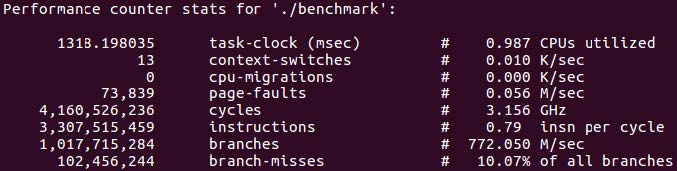
\includegraphics[width=0.9\textwidth]{content/1/chapter3/images/27.jpg}\\
圖3.27 - “假”分支的分支預測
\end{center}

分析器顯示與真正隨機分支一樣差的分支預測率。性能基準測試結果更證實了我們的猜想:

%\hspace*{\fill} \\ %插入空行
\begin{center}
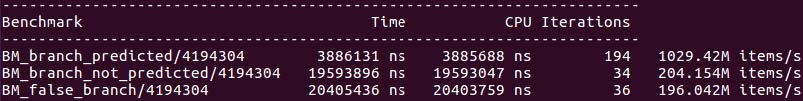
\includegraphics[width=0.9\textwidth]{content/1/chapter3/images/28.jpg}\\
圖 3.28
\end{center}

\textit{假}分支(不是真正的分支)的性能與真正隨機的、不可預測的分支一樣糟糕。

實際程序中,不應該出現這種不必要的條件語句。然而,常見的是複雜的條件表達式,其計算結果幾乎相同。例如,可能有一個條件很少為\texttt{false}:

\begin{lstlisting}[style=styleCXX]
if ((c1 && c2) || c3) {
	… true branch …
} else {
	… false branch …
}
\end{lstlisting}

幾乎一半的情況\texttt{c3}都是\texttt{true}。當\texttt{c3}為\texttt{false}時,\texttt{c1}和\texttt{c2}通常都為\texttt{true}。總條件應該容易預測,並且採用真分支。從處理器的角度來看,它不是一個單獨的條件,而是三個單獨的條件跳躍。如果\texttt{c1}為\texttt{true},那麼必須檢查\texttt{c2}。如果\texttt{c2}也為\texttt{true},則執行跳轉到真分支的第一個指令。如果\texttt{c1}或\texttt{c2}中的一個為\texttt{false},則檢查\texttt{c3}。如果為\texttt{true},則執行再次跳轉到\texttt{true}分支。

這個求值必須按特定順序完成,C++標準(以及在此之前的C標準)規定,像\&\&和||這樣的邏輯操作可以短路。當整個表達式的結果已知,對錶達式其餘部分的計算就應該停止。這在條件語句具有有副作用時尤為重要:

\begin{lstlisting}[style=styleCXX]
if (f1() || f2()) {
	… true branch …
} else {
	… false branch …
}
\end{lstlisting}

只有當\texttt{f1()}返回\texttt{false}時,才會調用函數\texttt{f2()}。前面的例子中,條件是簡單的布爾變量\texttt{c1}、\texttt{c2}和\texttt{c3}。編譯器已經知道沒有任何副作用,並且計算整個表達式不會改變可觀察行為。有些編譯器會做這種優化。如果\textit{假分支}基準測試使用這樣的編譯器,則會有良好的分支預測性能。但多數編譯器並沒有意識到這是一個問題(事實上,編譯器沒有辦法知道整個表達式的計算結果常為\texttt{true})。因此,這個優化需要開發手動完成。

假設開發者知道\texttt{if()}的兩個分支中有一個經常使用,例如:\texttt{else}分支可以對應錯誤情況,或其他一些必須正確處理,但在正常操作下不應出現的異常情況。假設做了正確的事情,並使用分析器進行了驗證,組成複雜布爾表達式的單個條件指令並沒有得到很好的預測。這時,如何優化代碼?

第一件事可能是將條件求值移出\texttt{if()}語句:

\begin{lstlisting}[style=styleCXX]
const bool c = (c1 && c2) || c3;
if (c) { … } else { … }
\end{lstlisting}

這肯定不會奏效,原因有二。首先,條件表達式使用邏輯\&\&和||操作,因此計算會短路,並且需要單獨和不可預測的分支。其次,編譯器可能會通過刪除不必要的臨時變量\texttt{c}來優化這段代碼,因此最終的代碼可能根本不會改變。

對條件變量數組進行循環時,可以使用類似的轉換。下面這段代碼很可能會受到分支預測的影響:

\begin{lstlisting}[style=styleCXX]
for (size_i i = 0; i < N; ++i) {
	if ((c1[i] && c2[i]) || c3[i]) { … } else { … }
}
\end{lstlisting}

但是,如果預先計算所有的條件表達式,並存儲在一個新數組中,大多數編譯器都不會幹掉這個臨時數組:

\begin{lstlisting}[style=styleCXX]
for (size_i i = 0; i < N; ++i) {
	c[i] = (c1[i] && c2[i]) || c3[i];
}
…
for (size_i i = 0; i < N; ++i) {
	if (c[i]) { … } else { … }
}
\end{lstlisting}

當然,用於初始化\texttt{c[i]}的布爾表達式,現在面臨著分支預測錯誤的問題,因此只有當第二個循環執行的次數比初始化循環多很多時,這種轉換才會有用。

通常有效的優化方法是用加法和乘法,或按位\&和|操作替換邏輯\&\&和||操作。這樣做之前,必須確定\&\&和||操作的參數是布爾值(值為0或1)而不是整數。即使值2解釋為真,表達式\texttt{2 \& 1}的結果與\texttt{bool(2) \& bool(1)}的結果也不相同。前者的計算結果為0(\texttt{false}),而後者預期的正確答案為1(或\texttt{true})。

我們可以在基準測試中比較這些優化代碼的性能:

%\hspace*{\fill} \\ %插入空行
\begin{center}
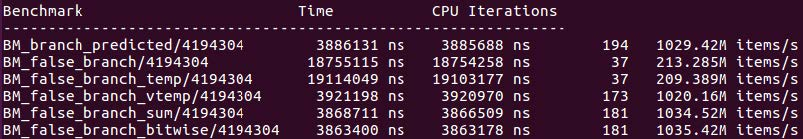
\includegraphics[width=0.9\textwidth]{content/1/chapter3/images/29.jpg}\\
圖 3.29
\end{center}

通過引入臨時變量\texttt{BM\_false\_branch\_temp}來優化\textit{假分支}的嘗試完全沒有效果。因為臨時向量的所有元素都為\texttt{true},這就是分支預測器所知道的(\texttt{BM\_false\_branch\_vtemp}),所以臨時向量給出了一個完全預測的分支的預期性能。用算術加法(+)或按位|替換邏輯||會產生類似的結果。

最後兩個轉換(使用算術或位操作,而不是邏輯操作)改變了代碼的含義:表達式中所有操作的參數都是求值的,並具有副作用。由編程者決定此更改是否會影響程序的正確性。如果副作用開銷特別大,那麼總體性能收益會是負的,例如:如果\texttt{f1()}和\texttt{f2()}非常耗時,那麼用等價的算術加法(\texttt{f1() + f2()})替換表達式\texttt{f1()|| f2()}中的操作會讓性能下降(即使它改善了分支預測)。

總的來說,沒有標準的方法來優化\textit{假分支}中的分支預測,這就是為什麼編譯器難進行有效的優化。開發者必須使用特定於問題的知識,例如:某個特定條件是否可能發生,並將其與分析結果相結合,以獲得最佳的解決方案。

瞭解了CPU操作如何影響性能,然後擴展到一個具體的和實際相關的例子中,並將這些知識應用於代碼優化。在結束本章之前,再來看一個優化示例。



























